\documentclass[11pt]{article}

\usepackage{fancyhdr}
\usepackage{pagecounting}
\usepackage[dvips]{color}
\usepackage{graphicx}
\usepackage{tikz}
\usetikzlibrary{arrows,positioning}
% Color Information from - http://www-h.eng.cam.ac.uk/help/tpl/textprocessing/latex_advanced/node13.html

% Trying to bold my name in the bib
\usepackage{xstring}
\def\FormatName#1{%
  \IfSubStr{#1}{Huff}{\textbf{#1}}{#1}%
}

\usepackage[left=1in, right=1in, top=1in, bottom=1in]{geometry}
\newcommand\bb[1]{\mbox{\em #1}}
\def\baselinestretch{1.1}
%\pagestyle{empty}
\newcommand{\hsp}{\hspace*{\parindent}}
\definecolor{gray}{rgb}{0.4,0.4,0.4}

\newcommand{\authorname}{Kathryn~D.~Huff }
\newcommand{\authoremail}{katyhuff@gmail.com}
\newcommand{\authorsite}{arfc.npre.illinois.edu}

\begin{document}

\pagestyle{fancy}
%\pagenumbering{gobble}
%\fancyhead[location]{text}
% Leave Left and Right Header empty.
%\lhead{}
%\rhead{}
\lhead{\textcolor{gray}{Investigator: Prof. \authorname\\Presenter: Mr. Andrei Rykhlevskii}}
\rhead{\textcolor{gray}{Advanced Reactors and Fuel Cycles\\}}
%\rhead{\textcolor{gray}{\thepage/\totalpages{}}}
\renewcommand{\headrulewidth}{0pt}
\renewcommand{\footrulewidth}{0pt}
\fancyfoot[C]{\footnotesize \textcolor{gray}{\authorsite}}

\paragraph{Research Goal}

The Advanced Reactors and Fuel Cycles (ARFC) group pursues improved safety and
sustainability of nuclear power. To do so, we model and
simulate the design, safety, and performance of advanced nuclear reactors.
Such reactors  involve tight coupling between physics such as thermal-hydraulic
phenomena, neutron transport, and fuel performance.

The current state of the art in advanced nuclear reactor simulation (e.g. the
CASL DOE innovation hub) is focused on traditional light water reactors.
The ARFC group seeks to extend that state of the art by enabling similarly high fidelity simulation of more advanced reactor designs through development of models and tools for representing unique materials, geometries, and physical phenomena. Current work includes extension
of the MOOSE framework to appropriately model coupled thermal-hydraulics and
neutronics of promising molten salt fuelled reactor designs.
ARFC develops physics kernel extensions and runs simulations using the highly
scalable, fully implicit, Multiphysics Object-Oriented Simulation Environment
(MOOSE) framework from Idaho National Laboratory.

Additionally, we have developed 
an online reprocessing model, SaltProc which includes fission product removal, fissile material 
separations, and refuelling for time dependent analysis of fuel-salt evolution. 
This tool relies on full-core high-fidelity Monte Carlo simulations perform depletion 
computations.

\paragraph{Role of Blue Waters}
Simulations which faithfully capture this coupling at realistic spatial and
temporal resolution are only possible with the aid of high performance
computing resources.  
To solve these large systems of partial differential
equations on a finite element mesh in a fully-coupled, implicit way, the MOOSE
framework was designed to take advantage of high performance computing
capability.  The framework conducts fully implicit physics coupling with
Newton-Krylov based solver methods and sophisticated automatic
adaptive meshing.  These simulations are memory intensive, so the exceptional
memory capability of the Blue Waters resource has been essential to performant
simulation times.

\paragraph{Progress}

Initial simulations of the Molten Salt Reactor Experiment and the conceptual 
Molten Salt Breeder Reactor have been conducted both locally on the desktop
computer scale and on Blue Waters with deterministic multiphysics and monte 
carlo methods respectively. Steady state, transient, and fuel cycle analysis 
simulations have been run in 2D as well as 3D. These simulations
have occupied up to many hundreds of nodes simultaneously and have resulted in 
rich datasets for use in reactor design and analysis. This talk will
describe how coupling between neutronics and thermal hydraulics have been
established in the Moltres and SaltProc tools, as well as the validation 
and verification efforts which have been completed.

The MOOSE framework is shown to scale very well up to 10,000 cores and Moltres 
scaling studies on Blue Waters have followed suit.
Transient and multi-scale simulations, which require greater capability per
simulation, can occupy thousands of CPU cores at a time. Such transient
simulations evaluate the safety performance of advanced reactors in severe
(beyond design basis) accidents.


Fuel cycle dynamics and quasi-equilibrium compositions were obtained 
from depletion and reprocessing simulations for a 10-year time frame. The 
MSBR full-core safety analysis was performed at the initial and equilibrium 
fuel salt compositions, for various reactor safety parameters such as effective 
multiplication factor, neutron flux distributions, temperature coefficients, 
rod worths, power and breeding distributions.


\paragraph{Potential Impact}
Current interest in advanced nuclear energy systems and molten salt reactor 
(MSR) concepts have reinforced interest in building tools to modeling these 
systems.  Detailed spatially and temporally resolved neutron flux and 
temperature distributions can improve designs, help characterize performance, 
inform reactor safety margins, and enable validation of numerical modeling 
techniques for unique physics.  Future work may include similarly challenging 
materials and geometries such as those in sodium cooled, gas cooled, and very 
high temperature reactor designs which also boast improved safety and 
sustainability.  

\begin{figure}[ht]
        \begin{center}
                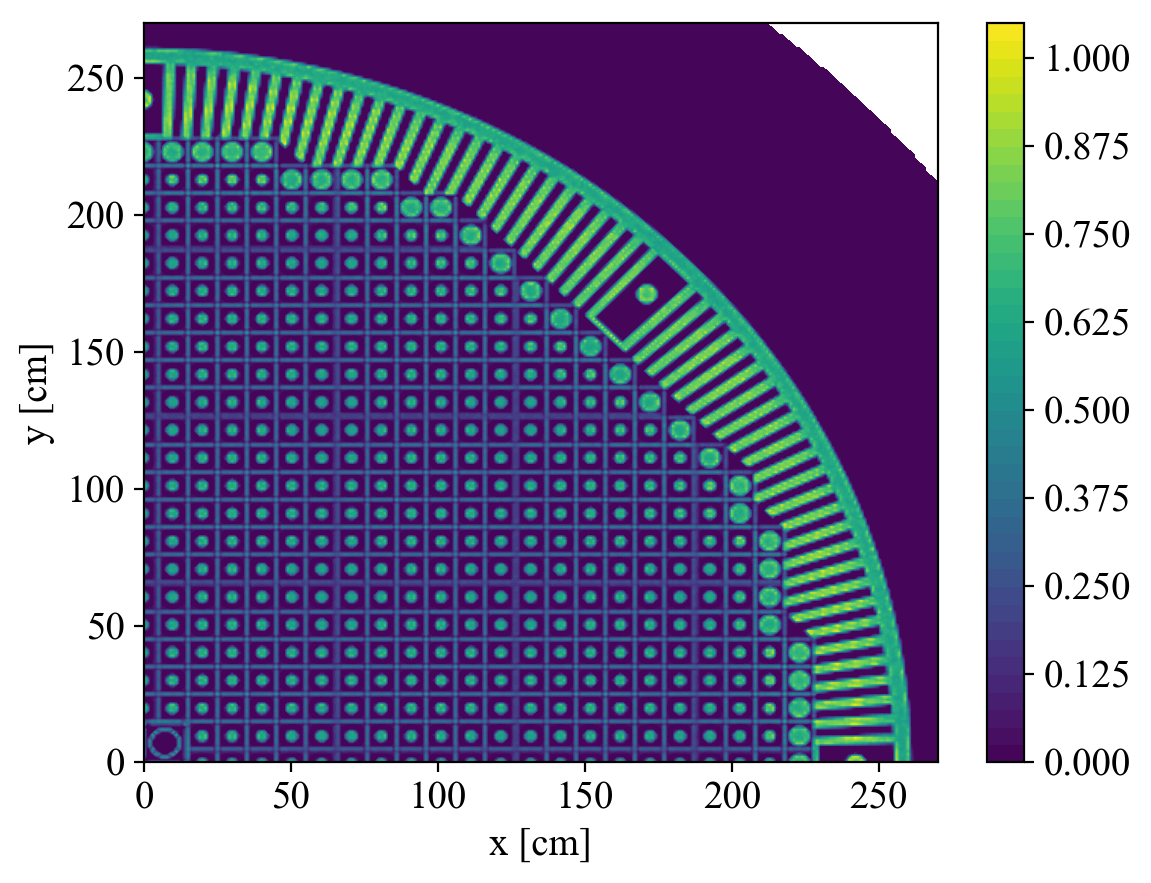
\includegraphics{breed_dens.png}
        \end{center}
        \caption{High fidelity monte carlo solutions of breeding density in the
                Molten Salt Breeder Reactor is at the heart of fuel cycle 
        analysis on Blue Waters.}
        \label{fig:breed_dens}
\end{figure}
\end{document}
